\tikzstyle{input}=[
    circle,
    very thick,
    minimum size=0.55cm,
    draw=black!80,
    fill=white!20
]

\tikzstyle{output}=[
    circle,
    very thick,
    minimum size=0.55cm,
    draw=black!80,
    fill=gray!20
]

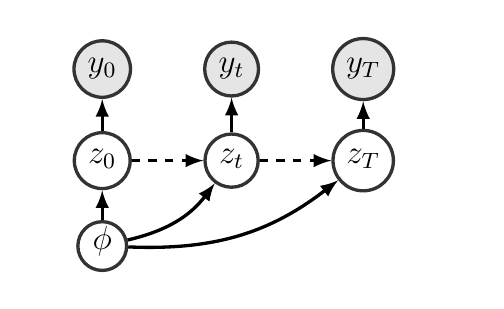
\begin{tikzpicture}[>=latex,text height=0.8ex,text depth=0.25ex]
	\matrix[row sep=0.35cm,column sep=0.45cm] {
		& % Y LAYER
		\node (y_0) [output]{\large $y_0$}; &   &
		\node (y_t) [output]{\large $y_t$}; &   &
		\node (y_T) [output]{\large $y_T$}; &   &
		\\ & % X LAYER
		\node (z_0) [input]{\large $z_0$}; &   &
		\node (z_t) [input]{\large $z_t$}; &   &
		\node (z_T) [input]{\large $z_T$}; &   &
		\\
        & \node (theta) [input]{\large $\phi$}; & \\
	};
	\path[->]
	% Horizontal connections
	(z_0) edge[very thick, dashed] (z_t)
	(z_t) edge[very thick, dashed] (z_T)

	% Connections from x to y
	(z_0) edge[very thick] (y_0)
	(z_t) edge[very thick] (y_t)
	(z_T) edge[very thick] (y_T)

  % Connections from pi to u
	(theta) edge[very thick] (z_0)
	(theta) edge[bend right=20, very thick] (z_t)
	(theta) edge[bend right=20, very thick] (z_T)
	;
\end{tikzpicture}
